In disem Abschnitt werden zuerst zwei M�glichkeiten f�r die Integration der Messung der Testabdeckung in das Framework vorgestellt. Nach einem Vergleich der beiden Ans�tze wird einen als L�sung ausgew�hlt

Die Aufgabe 

die SOAP-Nachrichten, die an Coverage Receiver gerichtet sind m�ssen dekodiert werden und  an den Servece (Mock) weitergeleitet werden.  

Ansatz1
Es kann ein spezieller Partner Track f�r den Service definiert und zu jedem TestCase zugeordnet werden. Zu jedem TestCase kann dann ein Thread gestartet werden, der die Coverage Nachrichten empf�ngt. Es reicht aus jedem TestCase aus. Es muss die Logik f�r den Manager der Marken implementiert werden. Daf�r kann entweder die receive Aktivit�t mehrmals hintereinander geschaltet werden, oder eine neue Aktivit�t, die alle Nachrichten akzeptiert.



 Das Framework dekodiert und leitet weiter , man braucht sich keine Gedanken zu machen. 

nachteil gr��ere Eingriffe in das Framework und an vielen Stellen:
\begin{itemize}
	\item beim Start jedes Testcases muss ein zus�tzliches Thread gestartet werden
	\item beim shutdown unber�cksichtigt 
	\item beim Auswerten des Ergebnissen muss dieser Thread unber�cksichtigt bleiben 
\end{itemize}



Ansatz2

Direkt nachdem Empfangen der Nachricht wird diese an den Receiver weitergeleitet. Dieser muss sich um die Dekodierung der SOAP Nachrichten k�mmern


Dadurch dass beim ersten Ansatz die ganze Funktionalit�t  der Kommunikation (der �bermittlung und Dekodierung der Nachrichten) durch das Framework erledigt werden erscheint diese M�glichkeit als eleganter. Aber Velangsamen





 
 \begin{figure}[htbp]
	\centering
		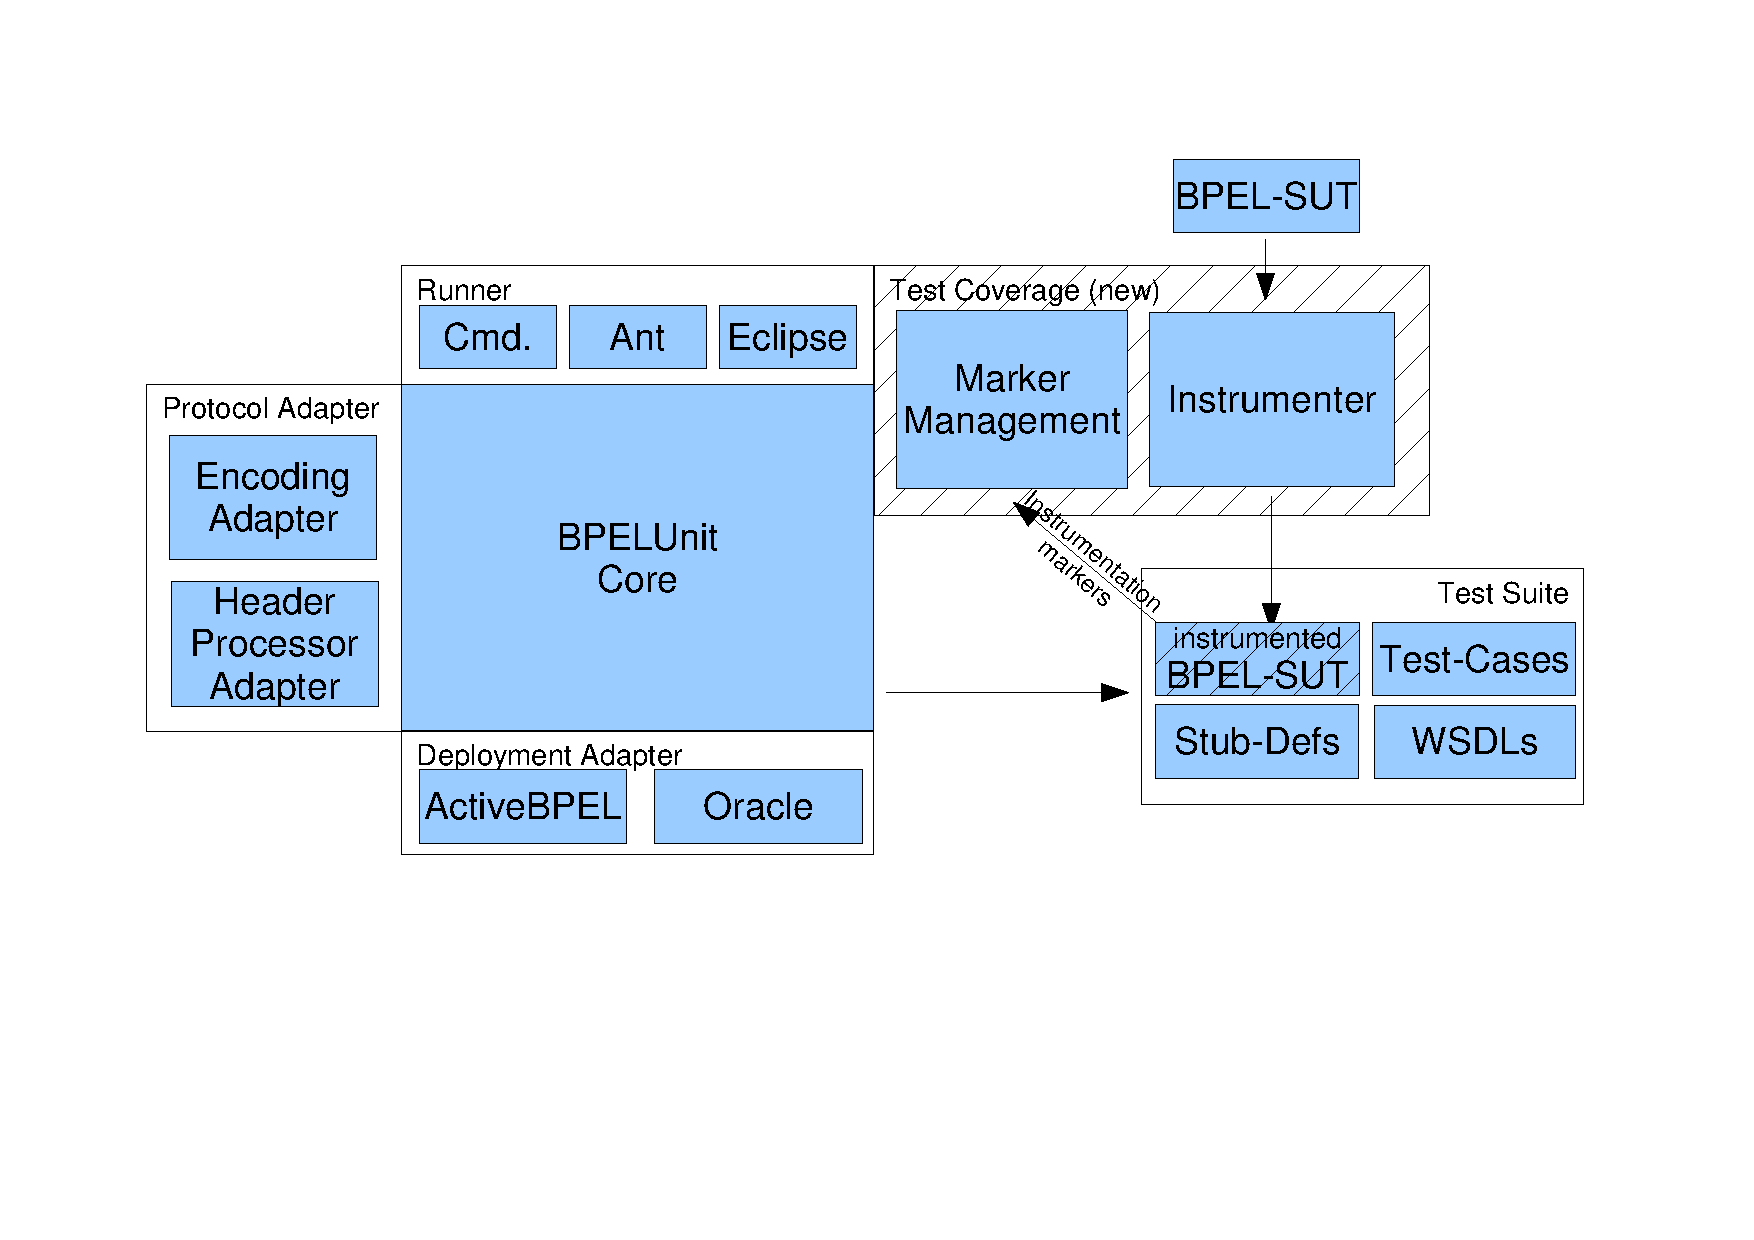
\includegraphics[width=0.9\textwidth]{bilder/bpelunit-architecture-with-coverage.pdf}
		\caption{Kontrollfluss eines BPEL Prozesses}
	\label{fig:ExamlpleBPELProzess}
\end{figure}

BPELUnit Framework wird erweitert durch hinzuf�gen einer Phase vor dem tats�chlichen Testen. In dieser Phase wird der BPEL Prozess annotiert , invoke-Aktivit�ten werdenhnzugef�gt. Diese Aktivit�teb sind Markierungen f�r jede Aktivit�t und jede M�glichkeit des Kontrollflusses. Die Marken haben eindeutige Identifizierungen, die verwendet werden umd die Relation zwischen Marken und Aktivit�ten bzw. dem Kontrollflu� 

Zur Laufzeit diese Aktivit��ten rufen ein Web Service des BPELUnit Frameworks . Bei diesen Aufrufen werden die Marken transportiert. , die signalisieren den Asf�hrungspfad zum BPELUnit Framework. Diesse Marken werden auf den BPEL Prozess abgebildet. Nach der Ausf�hrung k�nnen mit Hilfe der Marken und statischen Informationen �ber BPEL Prozess die Abdeckungsmetriken berechnet werden. Es ist ein neuer Modul hinzugekommen, der alle Aufgaben, die mit der Messung der Abdeckung zu tun haben, managt. So enth�lt dieser Modul einen Instrumentierer der den BPEL file analysiert und Annotationen hinzuf�gt. Der alte File wird durch den neuen ersetzt.  Zus�tzlich ist ein Web Service f�r das Empfangen von Marken in diesem Modul enhalten